\documentclass[11pt]{article}
\usepackage[a4paper,pdftex]{geometry}
\setlength{\oddsidemargin}{5mm}
\setlength{\evensidemargin}{5mm}
\usepackage[english]{babel}
\usepackage{amsmath,amsfonts,amsthm,amssymb}
\usepackage{graphicx}
\usepackage{fancyhdr}
\pagestyle{fancy}
\usepackage{subfig}
\usepackage{wrapfig}
\usepackage{comment}
\usepackage{url}
\urlstyle{same}
% Page numbering
\lhead{Dutch Nao Team - Explanatory paper Robotic Programming}
\rhead{page \thepage/5}
\cfoot{}
\rfoot{\thepage}

% TITLE FORMAT
\newcommand{\HRule}[1]{\rule{\linewidth}{#1}}

\makeatletter
\def\printtitle{
    {\centering \@title\par}}
\makeatother                  

\makeatletter
\def\printauthor{
    {\centering \large \@author}}
\makeatother

% TITLE
\title{
\HRule{0.5pt} \\
\LARGE \textbf{\textsc{Dutch Nao Team}}\\[0.5cm]
\normalsize \textsc{Explanatory paper about the educational value of Robotic Programming}\\
\texttt{http://www.dutchnaoteam.nl}
\normalsize
\HRule{2pt}\\ [0.5cm]
\normalsize
\today\\[1cm]
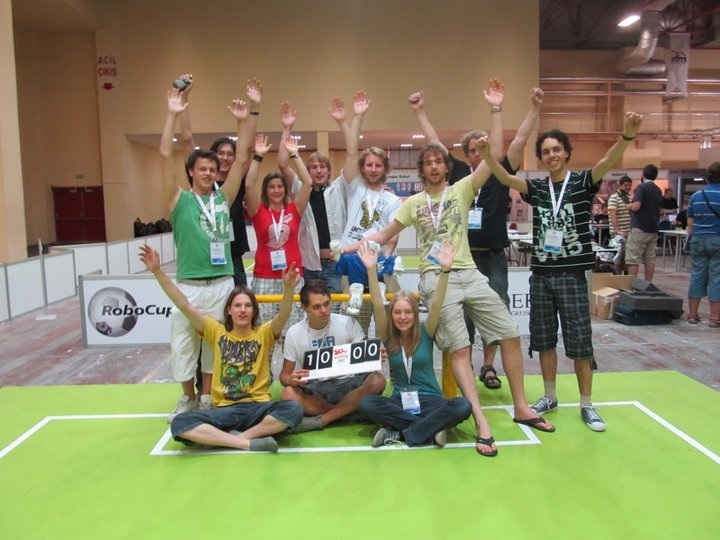
\includegraphics[width=0.8\textwidth]{team.jpg}
}

\author{
{C. R. Verschoor, D. S. ten Velthuis, A. C. Keune, I. G. Becht, M. de Jonge}\\ [0.2cm]
%\\
Dutch Nao Team\\
Faculty of Science\\
Universiteit van Amsterdam\\
\texttt{dutchnaoteam@googlegroups.com} \\
}


% BEGIN DOCUMENT
\begin{document}
\thispagestyle{empty}

% TITLE PAGE
\printtitle                  
\vfill
\printauthor
\newpage

% TABLE OF Contents
\setcounter{page}{1}
\normalsize
\tableofcontents
\newpage

% CONTENT
\section{Introduction}
The Dutch Nao Team was founded in 2010 by several Artificial Intelligence (AI) students in order to participate in the RoboCup. RoboCup is an international research and education initiative, attempting to foster Artificial Intelligence and Robotics research by providing a standard problem where a wide range of technologies can be integrated and examined, as well as being used for integrated project-oriented education.

The team consists of Artificial Intelligence Bachelor and Master students supported by senior staff-member Arnoud Visser. The Dutch Nao Team is the continuation of the Dutch Aibo Team; a cooperation of several Dutch universities, which began in the year 2004. The Dutch Aibo Team has been successful, both in the competition and with a number of publications [13, 7, 12, 11, 21, 10]
%(zoek deze referenties in technical report en gebruik ) . 

The official name of the project is `Robot Programming' and Bachelor of Science (BSc) students can attend it from the second year. The student will participate in the project during the whole year and will help write several publications. The final paper will be assessed and graded by the senior staff member. The project accomplished several results in the Standard Platform League and is a addition to the current AI curriculum as offered by the University of Amsterdam and we strive to become even better. This paper will give the reader some insight as to why the Dutch Nao Team is important for the University of Amsterdam, recent accomplishments and to share the future plans.
\section{Educational goals}
\subsection{Academic writing}
The Dutch Nao Team strives to document all progress made by its members by document these in a variety of reports. However, the most important is the annual Technical Report at the end of every academic year which contains a description of all the accomplishments of that year. It gives a short overview of competitions attended, code implemented and a guide on how to use the code and future goals in relation to the code. For reference we would direct you to the Technical Report of 2011 on the website\footnote{www.dutchnaoteam.com}.
 
All students have to document their progress, this consists of recognizing the problem, the tools that are used to solve the problem and the outcome of their solution. Students get a good sense of how to document their progress, but also how to show their end product to the rest of their teammates and to compare their improvement to the code of earlier years. 
Master students working with Dutch Nao Team will write their own thesis, which will be integrated in the final report.   

%Academisch schrijven: Qualificatie Paper, Team Description Paper, Technical Report, Open Challenge, Technical Challenge. Voetnoot in latex naar al deze papers
\subsection{Cooperation}
The Dutch Nao Team gives students a first experience with working in a large scale project in their bachelor. Each student can give his or hers preferred field to work in and will expand his or hers knowledge on this subject for a couple of months together with a small subgroup. In practice these tasks are divided into improving existing algorithms and implementing and experimenting with new ideas and additions. By working in a large group where there are multiple tasks to complete, the students learn working in a team environment and to communicate with their fellow programmers. They have to plan how they are going to handle their project by setting deadlines and to be able to present their findings and defend these to the rest of the group. The Dutch Nao Team strives to meet once every 2 weeks to talk about new developments in each project and to increase team building. 

The Dutch Nao Team differs from the currents projects presented throughout the Bachelor and Master because of the amount of time students spend on their Dutch Nao Team projects, a subject that is of interest to the student,  as well as working in a professional environment with professional work like feedback given from the other groups.

The team also offers a place to develop project management skills. Coordinating the groups, bringing exposure to Dutch Nao Team, collaborating with the university, companies and other teams, organizing trips around the world and thinking along about the future of RoboCup. 

\subsection{Experimentation Skills}
As most of our senior teammates have found out for themselves; not all theories work good in practice. A lot of the things we learn at school work great in a toy-like environment, where exercises most of the time deliver the result we would expect in the first place. However experimenting with this knowledge in real life can give quite different results. Working in the Dutch Nao Team gives that bit of practical experience where you often don't have enough time for in the day to day courses. This is an important part of research and gives students some new insight in how to think outside the box or combine different theories. It sharpens their intellectual thinking skills, all the while documenting all their progress.

\subsection{Programming}
Although we do some programming in the AI study, we do not get a lot of practical experience with large software projects in a team-like environment. Most programming exercises are small scaled and one-time only so you don’t get much real work-experience. The Dutch Nao team is quite a large-scaled software project where all code is combined in a multi-threaded system. Students need to think about the best structure for combining their code, what programming language to use, what code is most efficient and how to implement their code themselves. Most of the time new territory will be discovered for students while working with Dutch Nao Team. They learn a new programming language and deal with problems that most researchers and programmers will face as well, without being able to rely on a student assistant that knows all the answers in advance.

\section{Exposure}
The RoboCup is an inherently international event and this is a great opportunity for representing the Universiteit van Amsterdam. Throughout the year, several countries organize RoboCup Opens. These Opens are hosted all over the world, in places such as Germany, Italy and Iran. They’re attended by teams from all over the world, and are an excellent way of encouraging contact between universities. Once a year there’s a world championship, for which teams have to qualify. Simply qualifying for that is already an achievement in itself, and doing well is even more prestigious. 

All of these tournaments are an excellent place for the teams to expose themselves and the university it represents, which will gain a good reputation in the field of robotics. Currently being the only standard platform league team in the Netherlands, we’re one of the few places that have Nao robots, and the expertise to program them. This gives us the opportunity to give demonstrations or workshops at various events, or even at companies. For example, we’ve already given demonstrations at Nemo, open-door day at the Science Park and the bachelor-day, which attracted a large crowd and were received very well. It’s hard to talk about AI without mentioning robots sooner or later, and seeing our team can be very motivating to prospective AI students, making them more likely to choose to study at the University of Amsterdam.

As mentioned before we also release papers and publish\footnote{\url{http://www.dutchnaoteam.nl/index.php/publications/}} as much as we can. Giving even more credit to our co-operation.

\section{Vision of the future}
Dutch Nao Team aims for a full integration in the Artificial Intelligence study at the University of Amsterdam. Where it will become an elective one year project for BSc students and an elective Master thesis project. And on both accounts fully acknowledged in the study guide. Giving them the recognition that both parties need each other.

The University will be able to use Dutch Nao Team as promotional tool (think in terms of: study, research, unique selling point, link to partners, heb meer voordelen nodig). 

The more support Dutch Nao Team gets the more likely it will be able to end higher in the rankings of Robocup giving the University even more credit. And as the RoboCup is growing it’s getting more popular every year. It will only be a matter of time until the RoboCup teams will get world wide recognition when the progress of the league will get at its peak and they are able to defeat the Human Team that won the World Cup (scheduled for 2050). 

By that time Dutch Nao Team will be a cooperation between the University and Major Companies investing in Robot technology, giving the University a new revenue.
\end{document}
% END DOCUMENT​